\documentclass[10 pt,usenames,dvipsnames, oneside]{article}
\usepackage{../../../modelo-ensino-medio}



\begin{document}

\begin{center}
  \begin{minipage}[l]{3cm}

\includegraphics[width=2cm]{logo}    
\end{minipage}\hfill
\begin{minipage}[r]{.8\textwidth}
 {\Large \scshape Atividade: Triângulo de Sierpinski}  
\end{minipage}
\end{center}
\vspace{.2cm}

\ifdefined\prof
%Habilidades da BNCC
\begin{objetivos}
\item \textbf{EM13MAT508} Identificar e associar progressões geométricas (PG) a funções exponenciais de domínios discretos, para análise de propriedades, dedução de algumas fórmulas e resolução de problemas.
\end{objetivos}

%Caixa do Para o Professor
\begin{goals}
%Objetivos específicos
\begin{enumerate}
	\item Identificar progressões geométricas em construções geométricas.
\end{enumerate}

\tcblower

%Orientações e sugestões
\begin{itemize}
\item A Geometria Fractal pode ser utilizada para trabalhar alguns conceitos matemáticos de áreas como geometria plana e espacial, logaritmo, álgebra e progressões, sendo este último o conceito abordado nesta atividade. Caso seja de interesse explorar mais este assunto com os seus estudantes sugerimos essa referência \url{http://pmo.sbm.org.br/wp-content/uploads/sites/16/2018/11/pmo-sbm-v002-n001-cortes-e-antunes.pdf}.

\item Havendo possibilidade o software gratuito Xaos pode ser utilizado com a turma para explorar algumas das características dos fractais, em especial, a autossimilaridade. Ele pode ser baixado neste endereço \url{https://sourceforge.net/projects/xaos/}.

\end{itemize}
\end{goals}

\bigskip
\begin{center}
{\large \scshape Atividade}
\end{center}
\fi

Considere a seguinte construção geométrica. A partir de um triângulo equilátero - nossa figura inicial - determinamos os pontos médios de cada um dos seus lados e unimos esses pontos dois a dois formando um novo triângulo equilátero central que é retirado. Obtemos assim a segunda figura da construção que está ilustrada abaixo.

\begin{figure}[H]
\centering
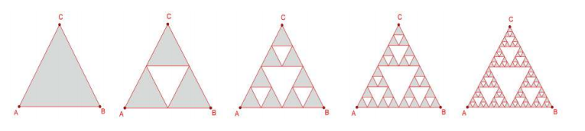
\includegraphics[width=.75\linewidth]{sierpinski.png}
\end{figure}

Seguimos adiante com a construção repetindo esse mesmo processo para cada um dos triângulos equiláteros sombreados que aparecem na figura 2. Obtemos assim a terceira figura da imagem acima. Seguindo com este processo recursivo indefinidamente obtemos uma figura conhecida como triângulo de Sierpinski, ele faz parte de um conjunto de objetos matemáticos chamados de fractais. Leia mais sobre eles no \textit{Você sabia} a seguir.

\begin{enumerate}

\item{}
Sem fazer contas, apenas olhando para o processo que descreve a construção do triângulo de Sierpinski, o que você diria sobre a área e o perímetro dele?

\item{}
Na tabela a seguir apresentamos os valores da área, do perímetro e da área esburacada da figura inicial e das duas primeiras iterações do processo de construção do triângulo de Sierpinski.

\begin{table}[H]
\centering
\setlength\tabulinesep{2.5pt}
\begin{tabu}{|c|c|c|c|}
\hline
\tmcol{1}{|l|}{} & \tcolor{Área} & \tcolor{Perímetro} & \tcolor{Área esburacada} \\ 
\hline
Figura inicial & A                                       & P                                       & 0                                                   \\ \hline
$1^a$ Iteração             & $A_1=\dfrac{3}{4}\cdot A$               & $P_1=\dfrac{3}{2}\cdot P$               & $B_1=\dfrac{1}{4}\cdot A$                           \\ \hline
$2^a$ Iteração             & $A_2=\left(\dfrac{3}{4}\right)^2\cdot A$ & $P_2=\left(\dfrac{3}{2}\right)^2\cdot P$ & $B_2=\dfrac{1}{4}\left[A+\dfrac{3}{4}\cdot A\right]$ \\ \hline
$3^a$ Iteração             & \multicolumn{1}{l|}{}                   & \multicolumn{1}{l|}{}                   & \multicolumn{1}{l|}{}                               \\ \hline
$4^a$ Iteração             & \multicolumn{1}{l|}{}                   & \multicolumn{1}{l|}{}                   & \multicolumn{1}{l|}{}                               \\ \hline
\end{tabu}
\end{table}

Complete as linhas da tabela com os valores da área, do perímetro e da área esburacada para a terceira e quarta iteração.

\item{}
Generalize as expressões que você encontrou para a área, o perímetro e a área esburacada a fim de obter expressões que representem os valores esperados para a n-ésima iteração.

\item{}
Utilize a expressão para a área esburacada que você encontrou no item anterior para concluir que a área do triângulo de Sierpinski é zero.

\end{enumerate}

\ifdefined\prof
\begin{solucao}

\begin{enumerate}
\item A área se aproxima de zero e o perímetro do infinito

\item \adjustbox{valign=t}
{
\setlength\tabulinesep{2.5pt}
\setlength\tabcolsep{2.5pt}
\begin{tabu} to \linewidth{|c|c|c|c|}
\hline
\tmcol{1}{|l|}{} & \tcolor{Área} & \tcolor{Perímetro} & \tcolor{Área esburacada} \\ 
\hline
Figura inicial & A & P & 0 \\ 
\hline

$1$\super{a} Iteração & 
$A_1=\dfrac{3}{4}\cdot A$ & 
$P_1=\dfrac{3}{2}\cdot P$ & 
$B_1=\dfrac{1}{4}\cdot A$ \\ 
\hline

$2$\super{a} Iteração & 
$A_2=\left(\dfrac{3}{4}\right)^2\cdot A$ & 
$P_2=\left(\dfrac{3}{2}\right)^2\cdot P$ & 
$B_2=\dfrac{1}{4}\left[A+\dfrac{3}{4}\cdot A\right]$ \\ 
\hline

$3$\super{a} Iteração & 
$A_3=\left(\dfrac{3}{4}\right)^3\cdot A$ & 
$P_3=\left(\dfrac{3}{2}\right)^3\cdot P$ & 
$B_3=\dfrac{1}{4}\cdot A\left[1+\dfrac{3}{4}+\bigg(\dfrac{3}{4}\bigg)^2\right]$\\ 
\hline

$4$\super{a} Iteração & 
$A_4=\left(\dfrac{3}{4}\right)^4\cdot A$ & 
$P_4=\left(\dfrac{3}{2}\right)^4\cdot P$& 
$B_4=\dfrac{1}{4}\cdot A\left[1+\dfrac{3}{4}+\bigg(\dfrac{3}{4}\bigg)^2+\bigg(\dfrac{3}{4}\bigg)^3\right]$\\ 
\hline
\end{tabu}
}

\item{}
$A_n=\left(\dfrac{3}{4}\right)^n\cdot A$

$P_n=\left(\dfrac{3}{2}\right)^n\cdot P$

$B_n=\dfrac{1}{4}\cdot A \cdot \left[1+\dfrac{3}{4}+\left(\dfrac{3}{4}\right)^2+ \dots +\left(\dfrac{3}{4}\right)^{n-1}\right]$

\item{}
A área esburacada no triângulo de Sierpinski será dada por

\[
\dfrac{1}{4}\cdot A \cdot \left[1+\dfrac{3}{4}+\left(\dfrac{3}{4}\right)^2+ \dots +\left(\dfrac{3}{4}\right)^{n-1}+ \cdots \right]
\]

Calculando a soma da PG infinita de razão $\dfrac{3}{4}$ que aparece dentro do colchete obtemos $\dfrac{1}{1-\frac{3}{4}}=4$, e portanto concluímos que a área esburacada será igual a $\dfrac{1}{4}\cdot A \cdot 4 = A$. Ou seja, o processo de construção do triângulo de Sierpinski nos leva ao final a uma figura com área igual a zero, uma vez que a área dos buracos será igual a área do triângulo que era nossa figura original.

\end{enumerate}

\end{solucao}
\fi

\end{document}